% !TEX TS-program = pdflatex
% !TEX encoding = UTF-8 Unicode

% This is a simple template for a LaTeX document using the "article" class.
% See "book", "report", "letter" for other types of document.

\documentclass[11pt]{article} % use larger type; default would be 10pt

\usepackage[utf8]{inputenc} % set input encoding (not needed with XeLaTeX)
\usepackage{graphicx}
\usepackage{subcaption}
\graphicspath{{./images/}}

%%% Examples of Article customizations
% These packages are optional, depending whether you want the features they provide.
% See the LaTeX Companion or other references for full information.

%%% PAGE DIMENSIONS
\usepackage{geometry} % to change the page dimensions
\geometry{a4paper} % or letterpaper (US) or a5paper or....
% \geometry{margin=2in} % for example, change the margins to 2 inches all round
% \geometry{landscape} % set up the page for landscape
%   read geometry.pdf for detailed page layout information

\usepackage{graphicx} % support the \includegraphics command and options

% \usepackage[parfill]{parskip} % Activate to begin paragraphs with an empty line rather than an indent

%%% PACKAGES
\usepackage{booktabs} % for much better looking tables
\usepackage{array} % for better arrays (eg matrices) in maths
\usepackage{paralist} % very flexible & customisable lists (eg. enumerate/itemize, etc.)
\usepackage{verbatim} % adds environment for commenting out blocks of text & for better verbatim
% These packages are all incorporated in the memoir class to one degree or another...

%%% HEADERS & FOOTERS
\usepackage{fancyhdr} % This should be set AFTER setting up the page geometry
\pagestyle{fancy} % options: empty , plain , fancy
\renewcommand{\headrulewidth}{0pt} % customise the layout...
\lhead{}\chead{}\rhead{}
\lfoot{}\cfoot{\thepage}\rfoot{}

%%% SECTION TITLE APPEARANCE
\usepackage{sectsty}
\allsectionsfont{\sffamily\mdseries\upshape} % (See the fntguide.pdf for font help)
% (This matches ConTeXt defaults)

%%% ToC (table of contents) APPEARANCE
\usepackage[nottoc,notlof,notlot]{tocbibind} % Put the bibliography in the ToC
\usepackage[titles,subfigure]{tocloft} % Alter the style of the Table of Contents
\renewcommand{\cftsecfont}{\rmfamily\mdseries\upshape}
\renewcommand{\cftsecpagefont}{\rmfamily\mdseries\upshape} % No bold!

%%% END Article customizations

%%% The "real" document content comes below...

\title{Design and Evaluation of a Machine Vision System for Identifying Cracked PV Panels}
\author{Jerome Wynne}
%\date{} % Activate to display a given date or no date (if empty),
         % otherwise the current date is printed 

\begin{document}
\maketitle

\section{Problem Description}

This work developed a system for automatically identifying cracks in PV panels from their 2D grayscale computed tomography images. 50 images were provided, of which 38 were deemed to be cracked. Several of these images are shown in Figure \ref{fig:sample_panels}.
\begin{figure}[h!]
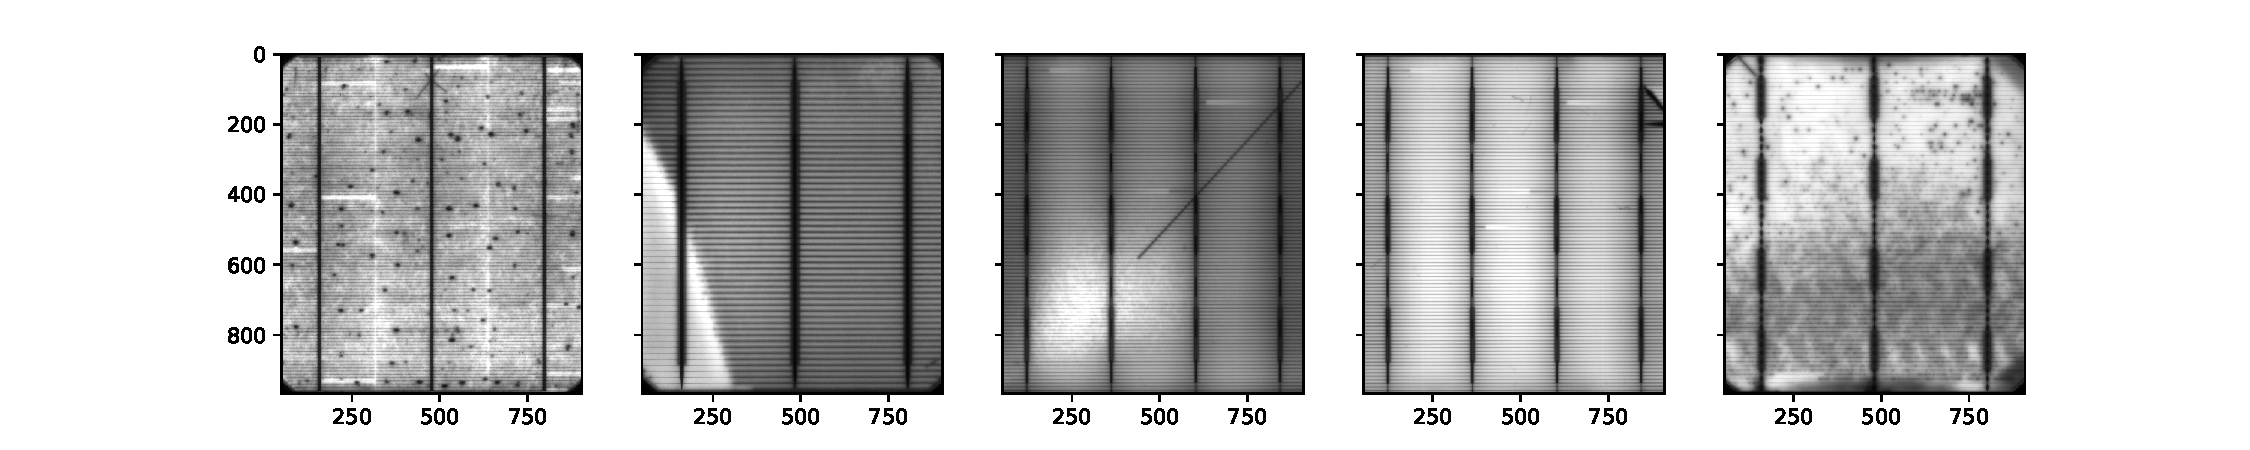
\includegraphics[width=\textwidth]{sample_panels.pdf}
\caption{Scans of the PV panels that were analyzed for damage. The first, third, fourth, and fifth panels from the left contain cracks. Pock-marks similar to those seen on the first panel were not regarded as cracks.}
\label{fig:sample_panels}
\end{figure}
 The median frame height for these images was 965 pixels; their width was similar.

 The criteria for labelling a given mark as a crack were as follows:
\begin{itemize}
	\item A dark line propagating diagonally for at least 50 pixels
	\item Was no more than 15 pixels in width (transverse to crack axis, see Figure \ref{fig:crack_width}
\end{itemize}
As can be seen in Figure \ref{fig:crack_v_scratch}, it was sometimes difficult to ascertain whether a given mark was a crack or a scratch. For the purposes of this work, the latter were considered to be fainter and wigglier - heuristic measures in the absence of any conveniently quantifiable differences. The labels themselves consisted of manually drawn binary masks, an example of which is shown in Figure \ref{fig:mask_example}. Each pixel in a mask was in effect indicators representing whether the associated image pixel was part of a crack. The masks were validated by a panel inspector. The centers of thick cracks were not labelled on the basis that they were too similar to other dark regions in the images (such as the vertical and horizontal bars).

\begin{figure}[h!]
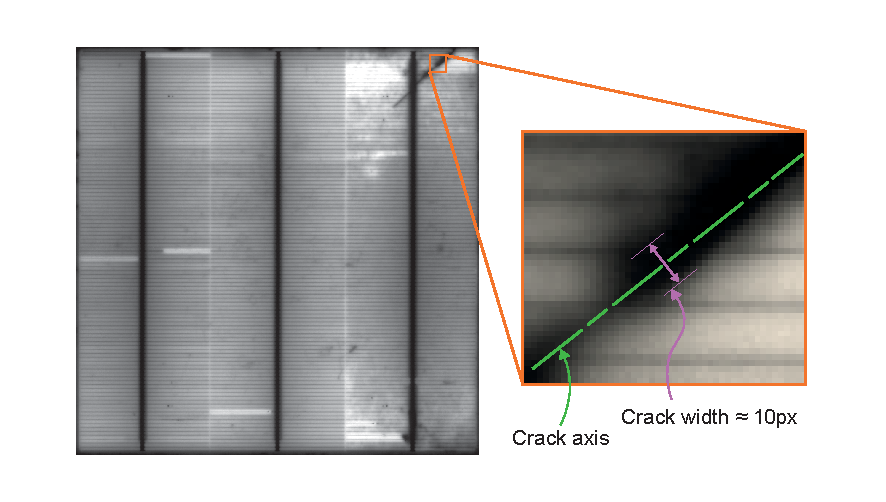
\includegraphics{crack_width.pdf}
\caption{Crack anatomy.}
\label{fig:crack_width}
\end{figure}

\begin{figure}[h!]
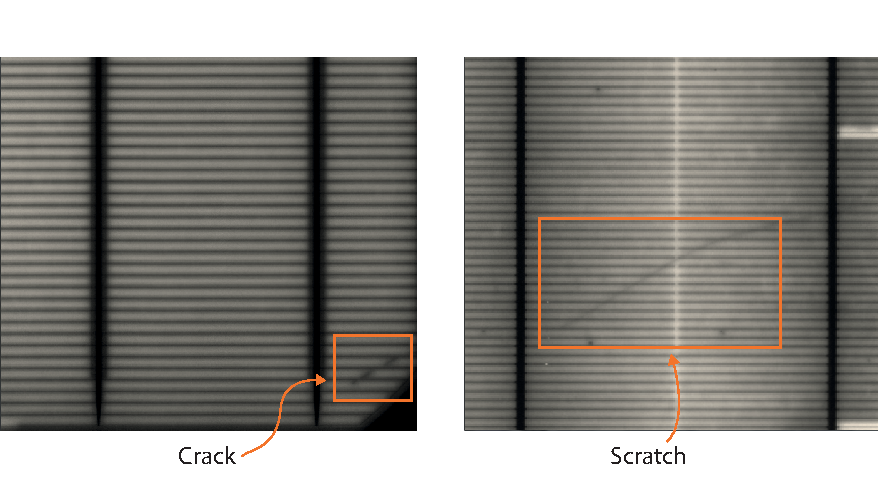
\includegraphics{crack_v_scratch.pdf}
\caption{Distinguishing between cracks and scratches was difficult in certain cases, making ground truth labels somewhat subjective.}
\label{fig:crack_v_scratch}
\end{figure}
Desirable properties of this sytem

\begin{figure}[h!]
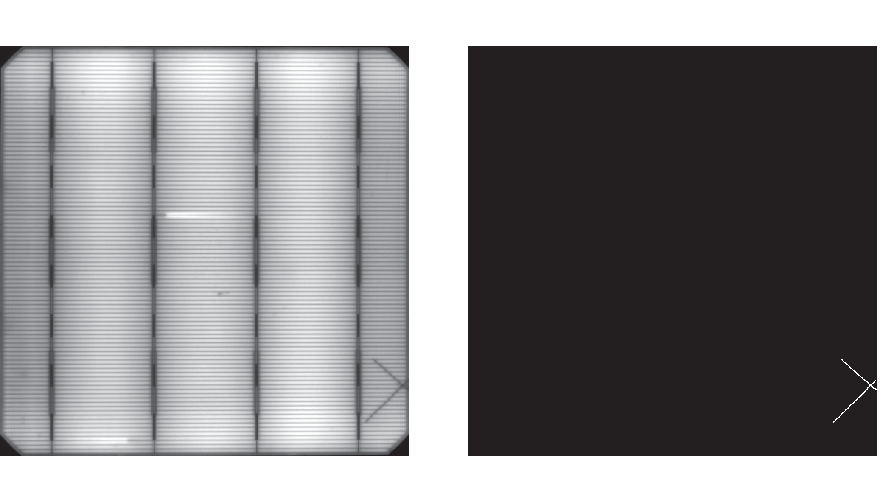
\includegraphics{mask_example.pdf}
\caption{A panel image and its associated set of labels.}
\label{fig:mask_example}
\end{figure}

\subsection{Pre-Processing}
Various filters were applied to the images in an attempt to emphasize cracks or suppress other features.

The most successful was as follows:
\begin{enumerate}
	\item Invert.
	\item Vertical Sobel filter.
	\item Gabor filter differencing.
\end{enumerate}
\begin{figure}
\centering
  	 \begin{subfigure}[b]{1\textwidth}
   	\includegraphics[width=\textwidth]{demo_images.pdf}
   	\caption{Raw images.}
   	\label{fig:b} 
	\end{subfigure}

  	 \begin{subfigure}[b]{1\textwidth}
   	\includegraphics[width=\textwidth]{sobelv.pdf}
   	\caption{Vertical Sobel filter.}
   	\label{fig:b} 
	\end{subfigure}
	
  	 \begin{subfigure}[b]{1\textwidth}
   	\includegraphics[width=\textwidth]{sobelv_gaborne.pdf}
   	\caption{Vertical Sobel filtering followed by a Gabor filter.}
   	\label{fig:d} 
	\end{subfigure}
	
	
  	 \begin{subfigure}[b]{1\textwidth}
   	\includegraphics[width=\textwidth]{sobelv_gabordiff.pdf}
   	\caption{Vertical Sobel filtering followed by a difference of two Gabor-filtered images.}
   	\label{fig:f} 
	\end{subfigure}
	
	\begin{subfigure}[b]{1\textwidth}
   	\includegraphics[width=\textwidth]{demo_masks.pdf}
   	\caption{Original image masks (i.e. ground truth).}
   	\label{fig:f} 
	\end{subfigure}
\caption{}
\end{figure}

\end{document}
